
\documentclass[crop,tikz]{standalone}
\usepackage[utf8]{inputenc}
\usepackage{tikz}
\usepackage{pgfplots}
\pgfplotsset{compat=newest}
\usepgfplotslibrary{groupplots}
\begin{document}
% This file was created by matplotlib2tikz v0.6.18.
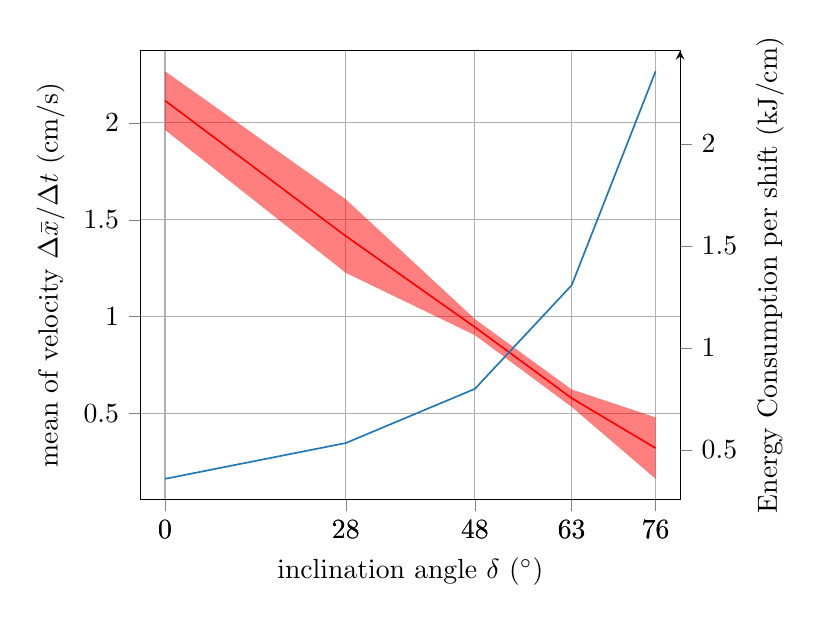
\begin{tikzpicture}

\definecolor{color0}{rgb}{0.12156862745098,0.466666666666667,0.705882352941177}

\begin{axis}[
tick align=outside,
tick pos=left,
x grid style={lightgray!92.02614379084967!black},
xlabel={inclination angle $\delta$ ($^\circ$)},
xmajorgrids,
xmin=-3.8, xmax=79.8,
xtick={0, 28, 48, 63, 76},
y grid style={lightgray!92.02614379084967!black},
ylabel={mean of velocity $\Delta \bar{x} / \Delta t$ (cm/s)},
ymajorgrids,
ymin=0.057264234671068, ymax=2.37204561366471
]
\path [fill=red, fill opacity=0.5] (axis cs:0,1.96397628120578)
--(axis cs:0,2.26682827825591)
--(axis cs:28,1.60563175285061)
--(axis cs:48,0.987303423028228)
--(axis cs:63,0.623881805839414)
--(axis cs:76,0.479558107289462)
--(axis cs:76,0.16248157007987)
--(axis cs:76,0.16248157007987)
--(axis cs:63,0.533745943535991)
--(axis cs:48,0.904218733296719)
--(axis cs:28,1.22619142742674)
--(axis cs:0,1.96397628120578)
--cycle;

\addplot [semithick, red, forget plot]
table [row sep=\\]{%
0	2.11540227973084 \\
28	1.41591159013868 \\
48	0.945761078162474 \\
63	0.578813874687702 \\
76	0.321019838684666 \\
};
\end{axis}

\begin{axis}[
axis y line=right,
tick align=outside,
x grid style={lightgray!92.02614379084967!black},
xmin=-3.8, xmax=79.8,
xtick pos=left,
xtick={0, 28, 48, 63, 76},
y grid style={lightgray!92.02614379084967!black},
ylabel={Energy Consumption per shift (kJ/cm)},
ymin=0.258188770852206, ymax=2.45528543159973,
ytick pos=right
]
\addplot [semithick, color0, forget plot]
table [row sep=\\]{%
0	0.358056800886184 \\
28	0.533417870806547 \\
48	0.798977935433184 \\
63	1.30710073128005 \\
76	2.35541740156575 \\
};
\end{axis}

\end{tikzpicture}
%% End matplotlib2tikz content %% 
\end{document}